\documentclass[aspectratio=169]{beamer} % 16:9 aspect ratio for modern screens

% Theme settings
\usetheme{metropolis} % Minimalist theme
\usefonttheme{professionalfonts} % Font theme

% Packages
\usepackage[T1]{fontenc}   % Font encoding
\usepackage[ngerman]{babel} % German language
\usepackage[sfdefault]{FiraSans} % For FiraSans font
\usepackage[backend=biber, style=authoryear, sorting=nyt]{biblatex} % For bibliography
\usepackage{csquotes} % Recommended for biblatex with babel/polyglossia
\usepackage{textgreek} % Greek letters in text mode (aus references von Citavi)


\usepackage{graphicx}       % For including images
\usepackage{amsmath, amssymb} % For math symbols

% Bibliography settings
\addbibresource{references.bib} % Path to the bibliography file

% custom Citation commands
\DeclareCiteCommand{\citeauthortitle}
  {\usebibmacro{prenote}}
  {\usebibmacro{citeindex}%
   \printnames{labelname}%
   \setunit{\addcolon\space}% <- Hier wird das Trennzeichen ":" hinzugefügt
   \printfield{title}}
  {\multicitedelim}
  {\usebibmacro{postnote}}

\DeclareCiteCommand{\parenciteauthortitle}
  {\usebibmacro{prenote}}
  {\bibopenparen\usebibmacro{citeindex}%
   \printnames{labelname}%
   \setunit{\addcolon\space}% <- Hier wird das Trennzeichen ":" hinzugefügt
   \printfield{title}\bibcloseparen}
  {\multicitedelim}
  {\usebibmacro{postnote}}

% Title page settings
\title{Hadronen im Quarkmodell}
\subtitle{Eine physikalische Betrachtung}
\author{Florian Adamczyk}
\date{\today}

\begin{document}
    
    % Title Slide
    \begin{frame}\titlepage\end{frame}
    
    % Table of Contents
    \begin{frame}{Inhaltsverzeichnis}
        \tableofcontents
    \end{frame}
    
    % Section: Einführung
    \section{Einführung}
    \begin{frame}{Einführung}
        \begin{block}{Ziel der Präsentation}
            \begin{itemize}
                \item Vorstellung der Grundlagen des Quarkmodells
                \item Beschreibung der Hadronenstruktur
                \item Diskussion aktueller Herausforderungen
            \end{itemize}
        \end{block}
        \begin{figure}
            \centering
            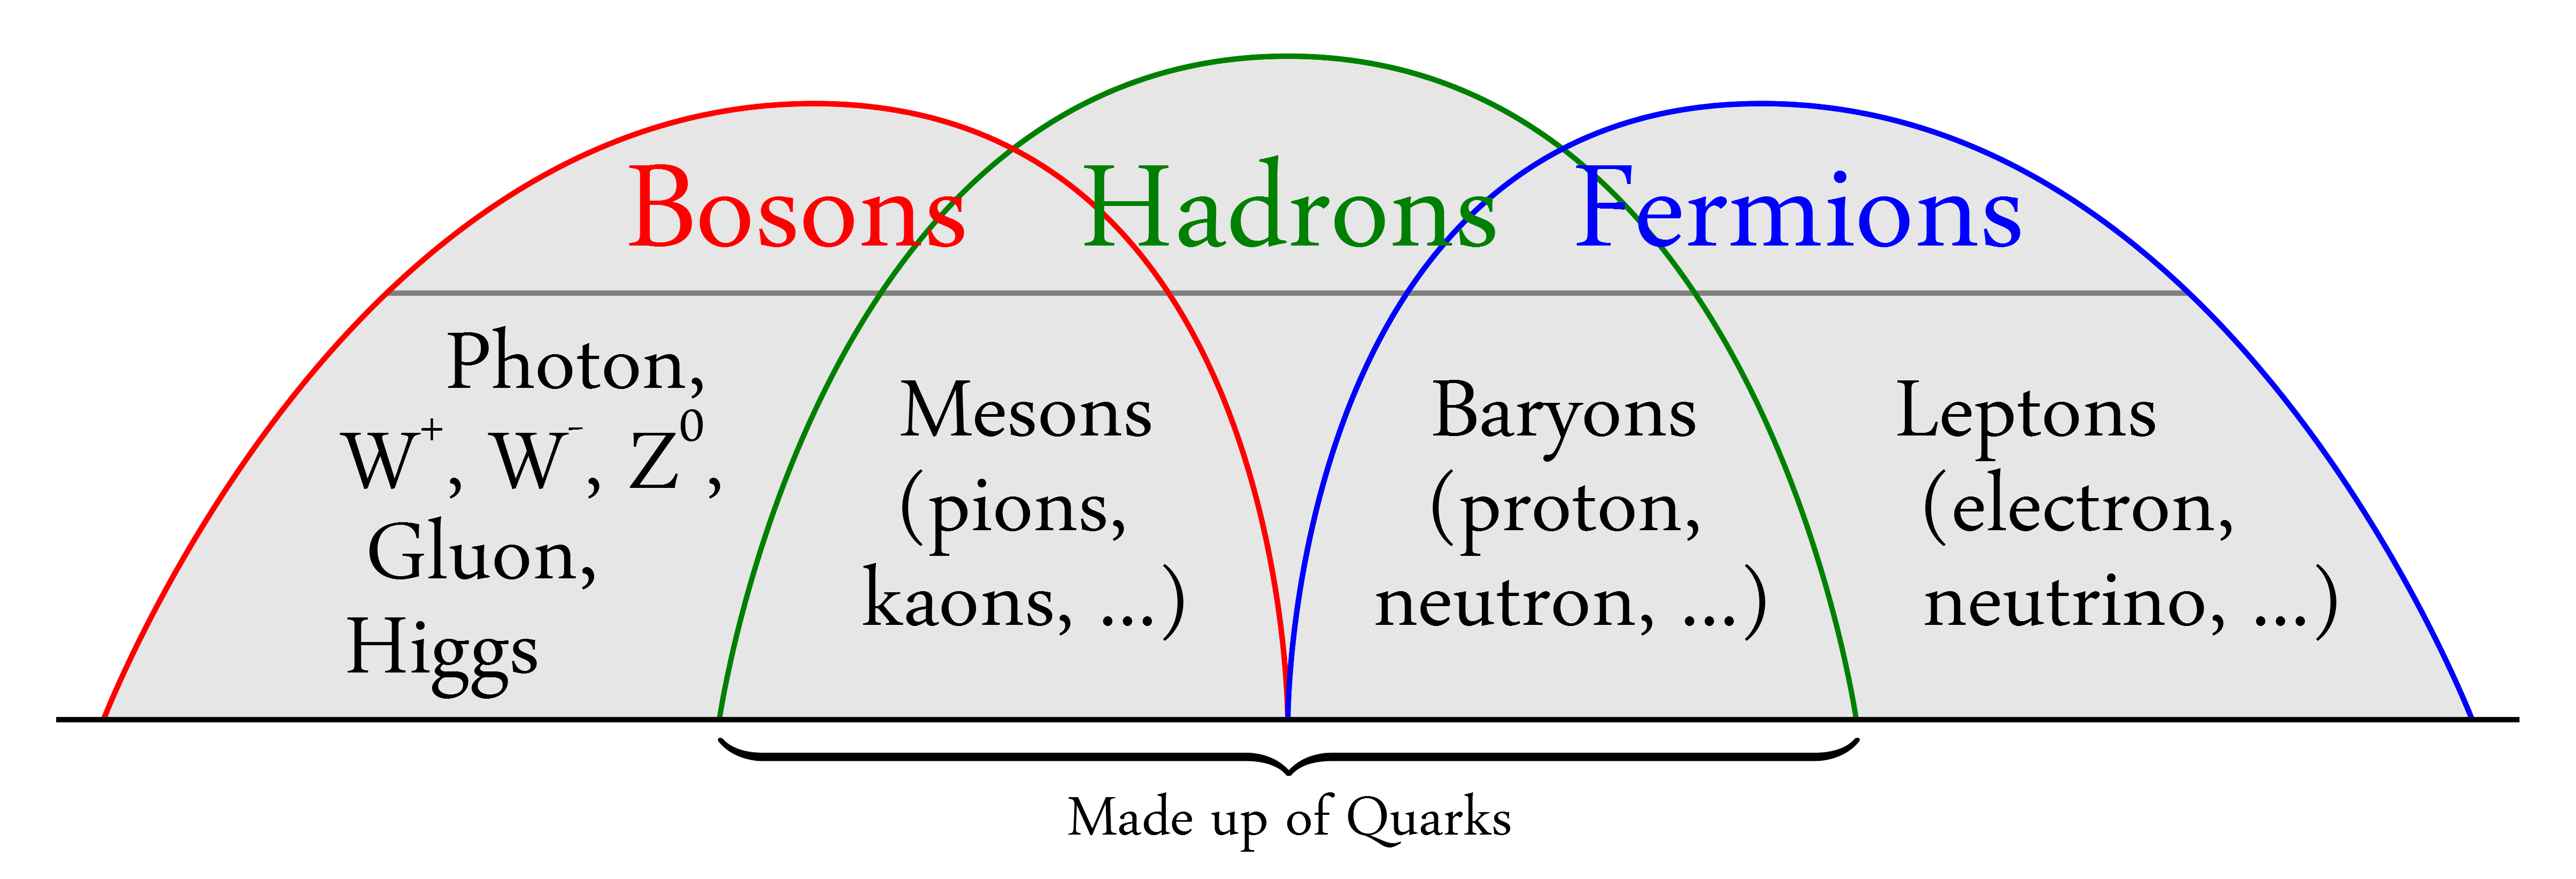
\includegraphics[width=0.6\linewidth]{Bosons-Hadrons-Fermions-RGB-png2.png}
        \end{figure}
    \end{frame}
    
    % Section: Theoretische Grundlagen
    \section{Theoretische Grundlagen}
    \begin{frame}{Quarkmodell: Ein Überblick}
        \begin{itemize}
            \item Quarks als fundamentale Bausteine
            \item Drei Farbladungen: Rot, Grün, Blau
            \item Austausch von Gluonen $\Rightarrow$ starke Wechselwirkung
        \end{itemize}
        \begin{equation*}
            F = \frac{Gm_1m_2}{r^2} % Beispiel für eine Formel
        \end{equation*}
    \end{frame}
    
    \begin{frame}{Hadronenklassen}
        \begin{block}{Baryonen}
            \begin{itemize}
                \item Drei Quarks
                \item Beispiele: Proton, Neutron
            \end{itemize}
        \end{block}
        \begin{block}{Mesonen}
            \begin{itemize}
                \item Ein Quark und ein Antiquark
                \item Beispiele: Pionen, Kaonen
            \end{itemize}
        \end{block}
    \end{frame}
    
    % Section: Experimentelle Beobachtungen
    \section{Experimentelle Beobachtungen}
    \begin{frame}{Nachweis von Quarks}
        \begin{figure}
            \centering
            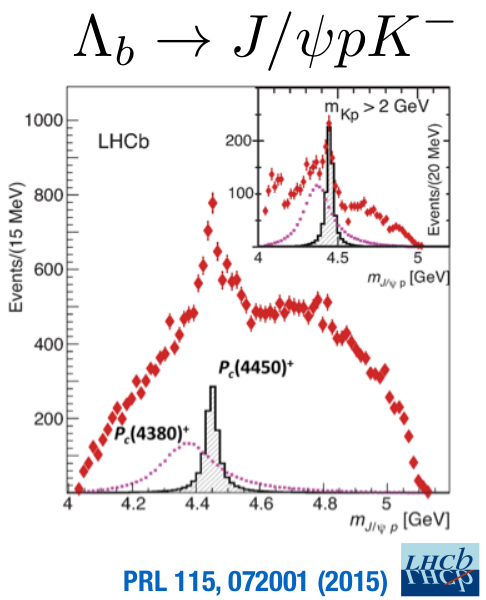
\includegraphics[width=\linewidth, height=0.5\textheight, keepaspectratio]{lhcb-pc4450.png} %\caption{Streuexperiment zur Quarkstruktur}
        \end{figure}
        \begin{itemize}
            \item Streuexperimente als zentrale Methode
            \item Nachweis von Quark-Ladungen
        \end{itemize}
    \end{frame}
    
    % New Slide with Citations
    \begin{frame}{Wichtige Quellen}
        \begin{itemize}
          \item Test
            \item Die Grundlagen des Quarkmodells wurden von Gell-Mann (1964) und Zweig (1964a, 1964b) entwickelt~\cite{GellMann.1964, Zweig.1964, Zweig.1964b}.
            \item Amsler et al. (2017) bieten eine umfassende Übersicht über das Quarkmodell~\cite{C.Amsler.2017}.
            \item Die Entdeckung von Pentaquark-Zuständen wurde von Aaij et al. (2015, 2019) berichtet~\cite{Aaij.2019}.
            \item Wikipedia bietet zugängliche Erklärungen zu Hadronen und dem Standardmodell~\cite{Wikipedia.Hadron, Wikipedia.Standardmodell}.
        \end{itemize}
    \end{frame}
    
    % Section: Zusammenfassung
    \section{Zusammenfassung}
    \begin{frame}{Schlussfolgerungen}
        \begin{itemize}
            \item Hadronen sind komplexe Strukturen aus Quarks
            \item Fortschritte in der Theorie und Experimente erforderlich
            \item Bedeutung des Quarkmodells für die moderne Physik
        \end{itemize}
    \end{frame}
    
    % Thank You Slide
    \begin{frame}{Vielen Dank!}
        \begin{center}
            \Huge Fragen?
        \end{center}
    \end{frame}

    % Bibliography
    \begin{frame}[allowframebreaks]{Literaturverzeichnis}
        \printbibliography[nottype=unpublished]
    \end{frame}

\end{document}
